\documentclass[12pt, aspectratio=43]{beamer} 

\input{package.tex} % 載入封包與文檔配置

% Title, Subtitle, Author, Institute, Date
\title[\textbf{Week 7 Report}]{Week 7 Report}
\author[Chen, Pin-Jui]{Chen, Pin-Jui}
\date{\today}

\begin{document}
	
	% Title page frame
	\begin{frame}
		\titlepage
	\end{frame}
	
	% Index
	\section{Single Cell Workflow}
	
	\begin{frame}
		\tableofcontents[currentsection,]
	\end{frame}
	\begin{frame}
		\begin{figure}[h!]
			\centering
			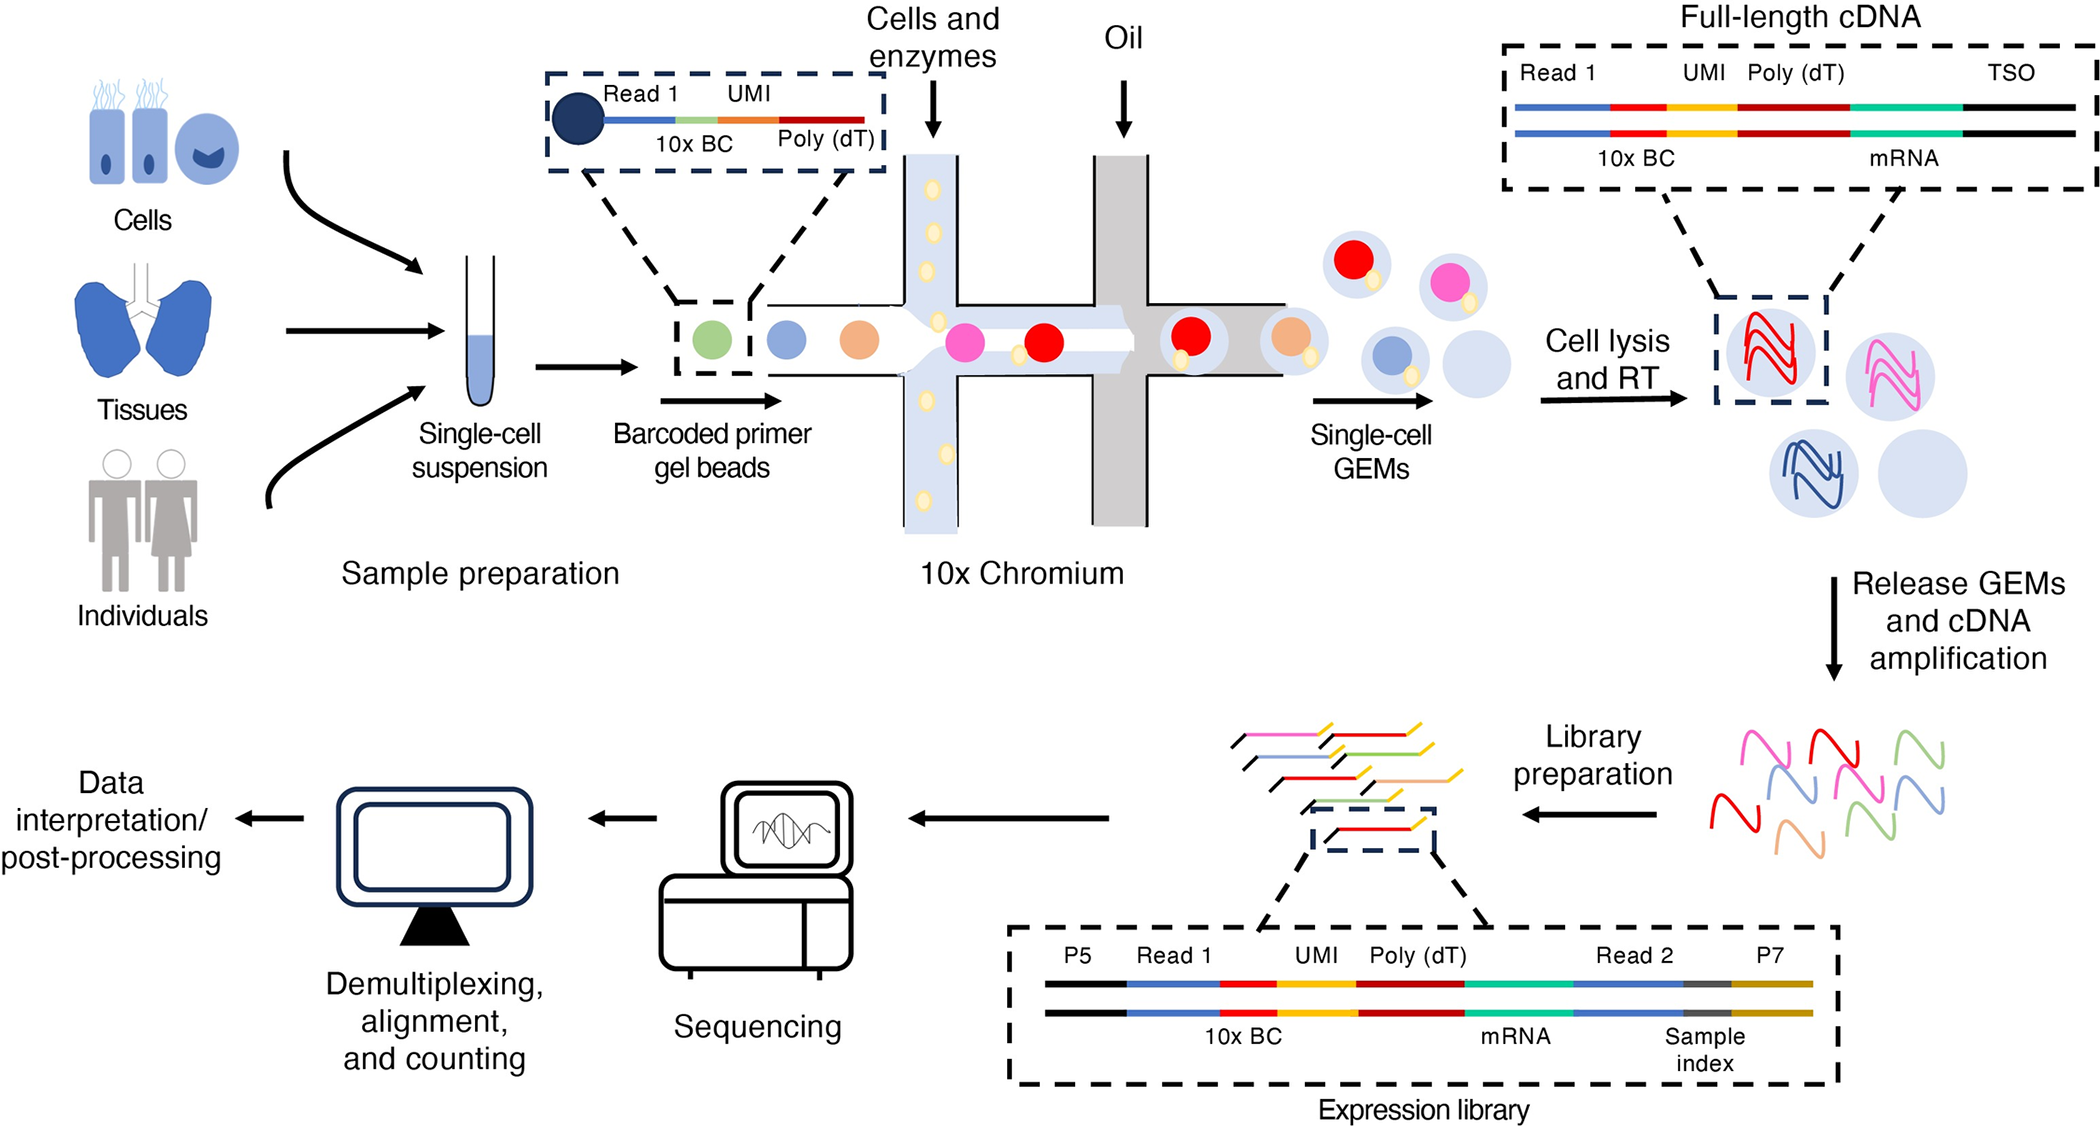
\includegraphics[width=\linewidth]{Figure/single_cell_work.png}
		\end{figure}
	\end{frame}
	
	\begin{frame}{Barcode}
		\begin{enumerate}
			\item Read 1
			\item Cell Barcode
			\item UMI
			\item Poly(dt)
		\end{enumerate}
	\end{frame}
	
	\begin{frame}{Feature Barcode}
		\begin{enumerate}
			\item Antibody Capture (cell surface protein measurement): A method to label cell surface proteins using a specific protein binding molecule, such as an antibody conjugated to a Feature Barcode oligonucleotide. 
			
			\item CRISPR Guide Capture: A method to analyze gene expression changes caused by the presence of CRISPR perturbations. The assay captures the full transcriptome and transfected guide RNAs from the same cell to correlate changes in the transcriptome to CRISPR perturbations. 
			
			\item 3' Cell Multiplexing: A method to label a given cell (or nuclei) sample with a molecular tag and subsequently pooling this sample with other labeled samples.
		\end{enumerate}
	\end{frame}
	
	
	\begin{frame}{Feature Barcode Technology}
		\begin{figure}[h!]
			\centering
			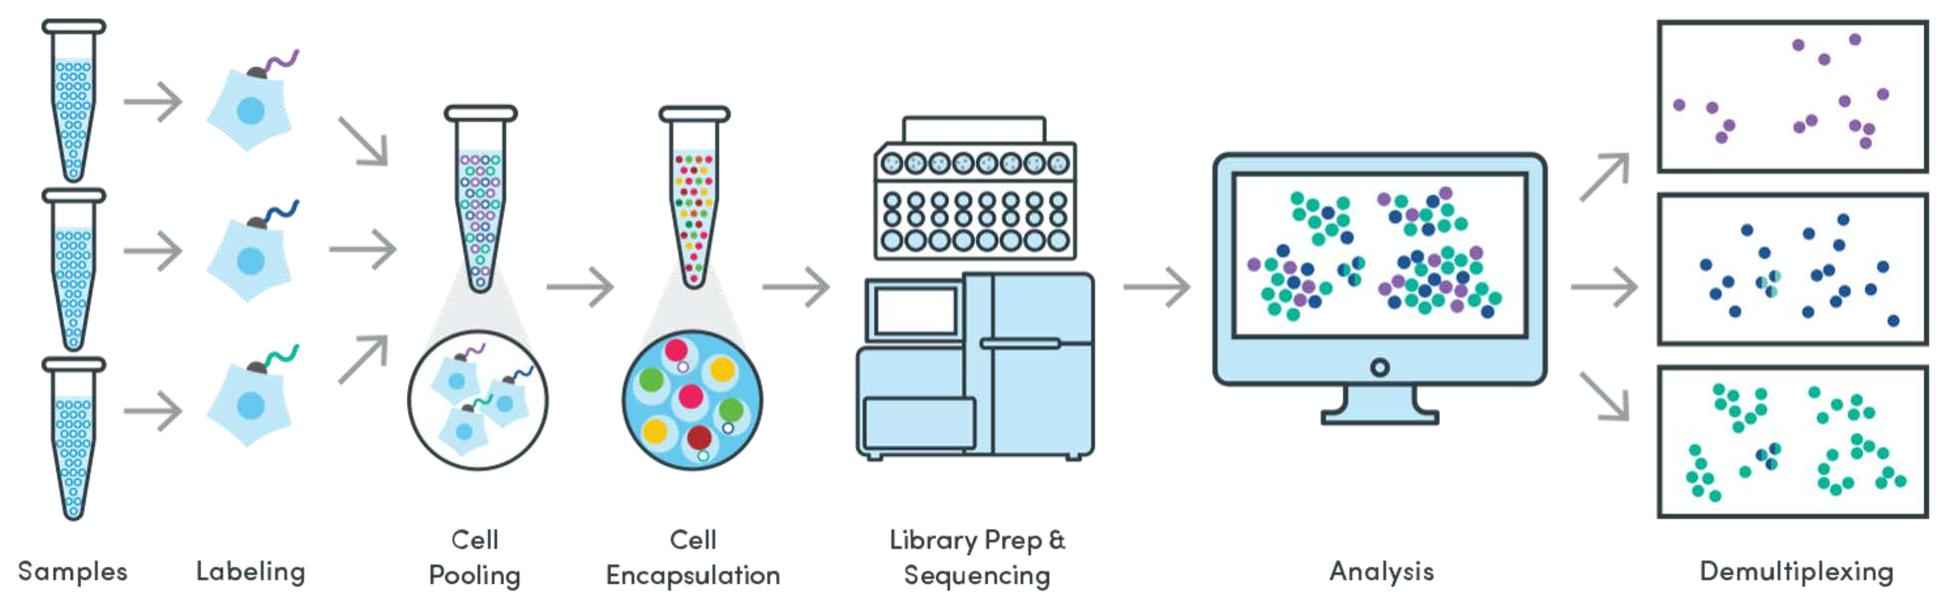
\includegraphics[width=\linewidth]{Figure/Feature_barcode.png}
		\end{figure}
	\end{frame}
	
	\begin{frame}{Gene Expression \& Feature Barcode}
		\begin{figure}[h!]
			\centering
			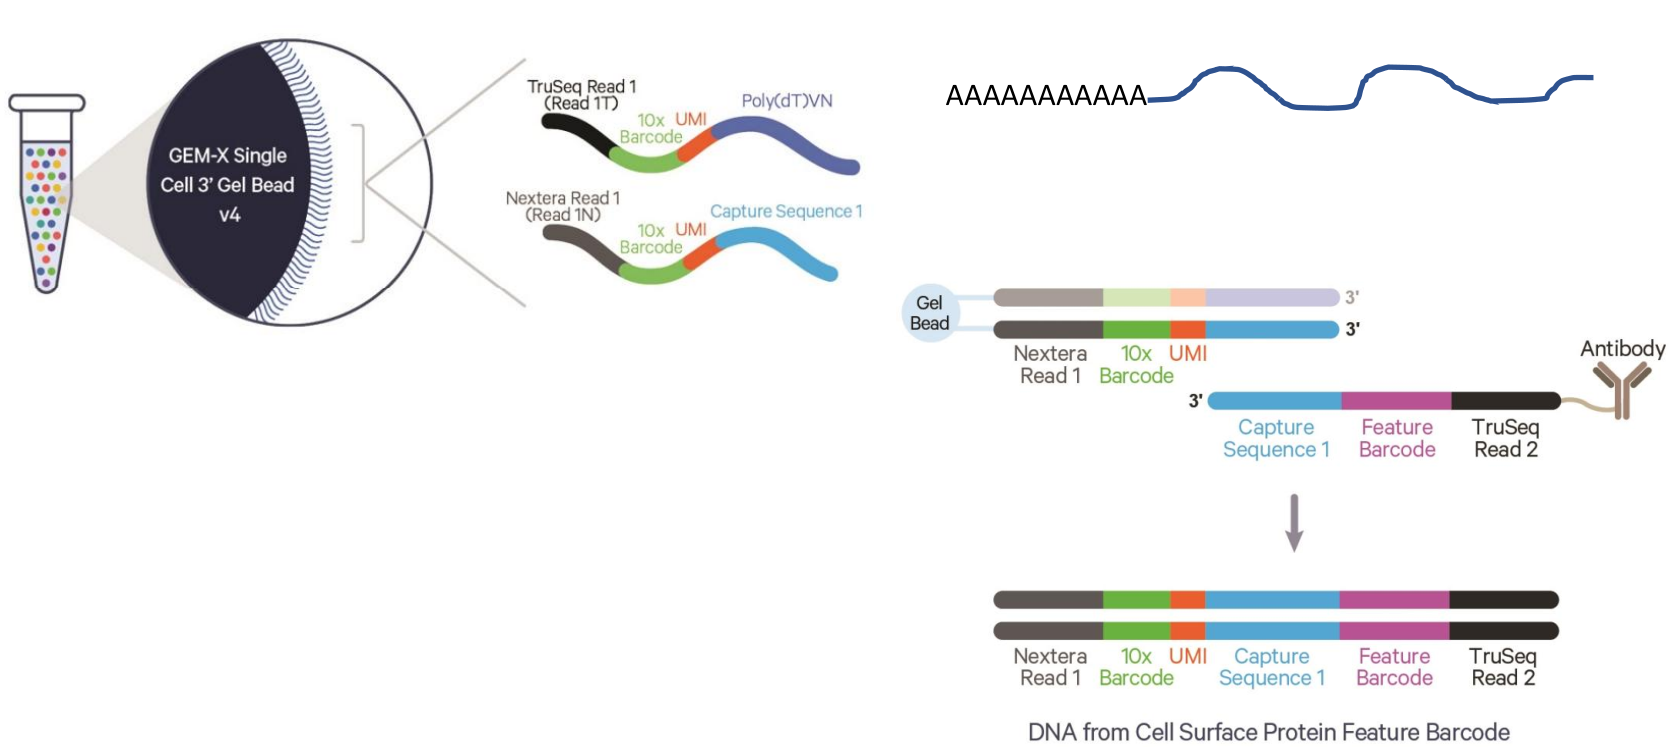
\includegraphics[width=\linewidth]{Figure/Gene_Expression.png}
		\end{figure}
	\end{frame}
	
	\begin{frame}{Gene Expression \& Feature Barcode}
		\begin{figure}[h!]
			\centering
			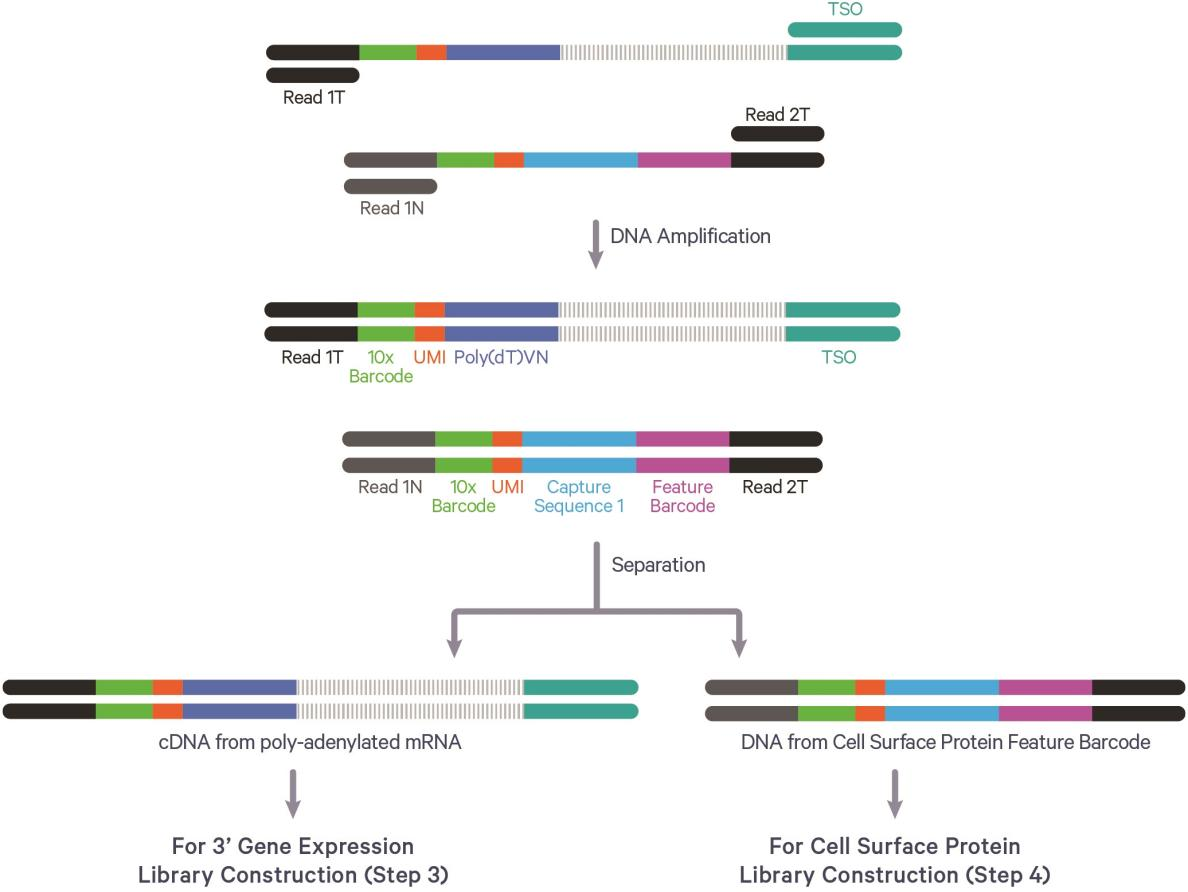
\includegraphics[width=0.8\linewidth]{Figure/Gene_Expression_2.png}
		\end{figure}
	\end{frame}
	
	
	\begin{frame}{Gene Expression \& Feature Barcode}
		\begin{figure}[h!]
			\centering
			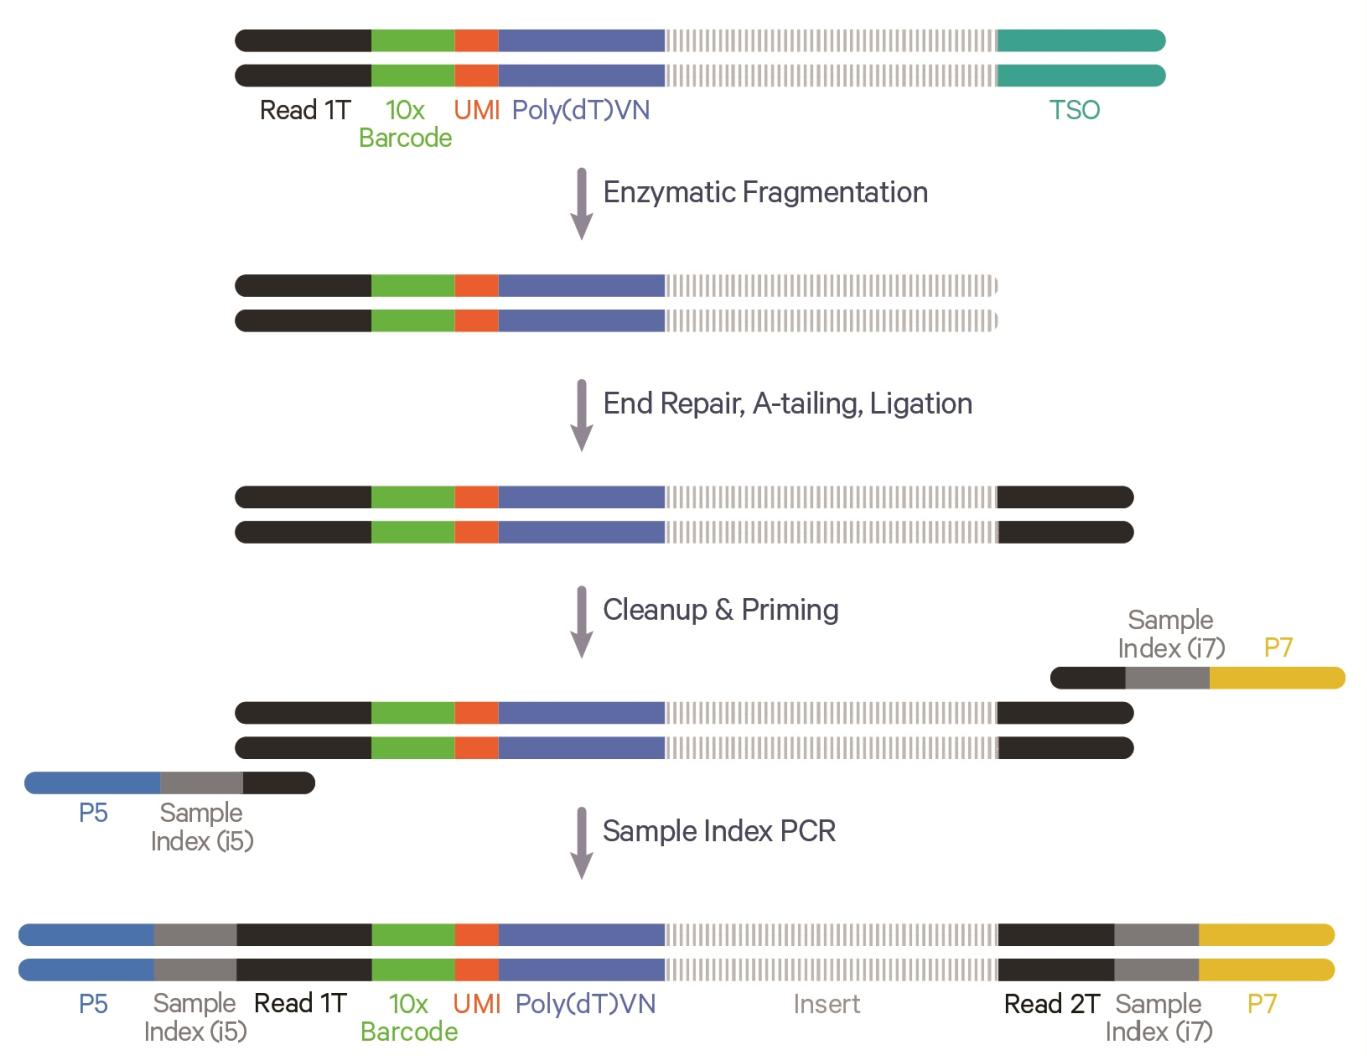
\includegraphics[width=0.8\linewidth]{Figure/Gene_Expression_3.png}
		\end{figure}
	\end{frame}
	
	\begin{frame}{Flex Gene Expression \& Feature Barcode}
		\begin{figure}[h!]
			\centering
			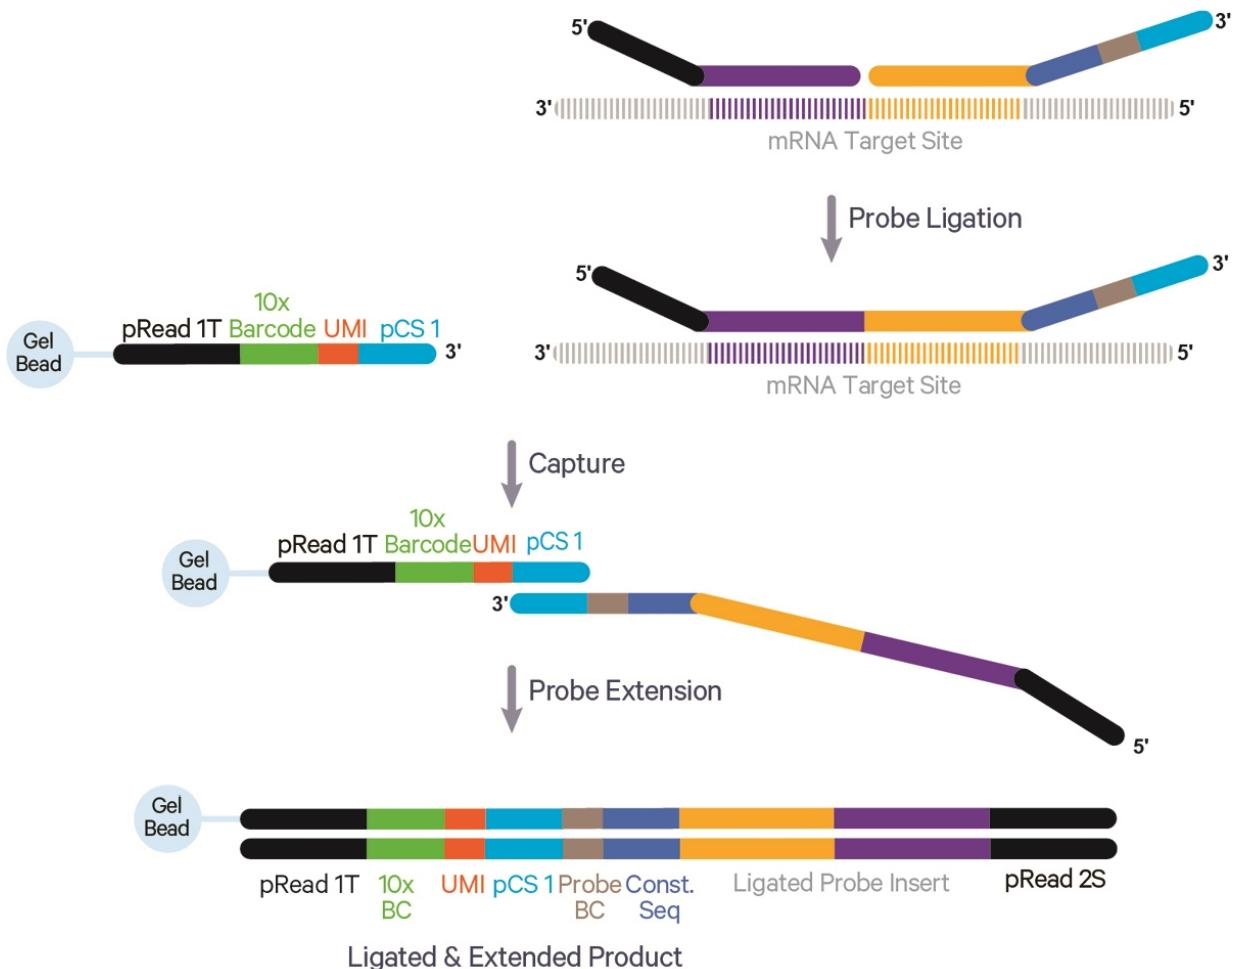
\includegraphics[width=0.8\linewidth]{Figure/Flex.png}
		\end{figure}
	\end{frame}
	
	
	\section{Bulk COAD GSEA}
	
	\begin{frame}
		\tableofcontents[currentsubsection,]
	\end{frame}
	
	\begin{frame}{GSEA}
		Use \textbf{KEGG gene sets}
		\vskip 0.2cm
		Number of genes used in GSEA: 17313
		\vskip 0.2cm
		Compare \textbf{logFC} and \textbf{t-value} sorting (Tumor vs Normal).
		\vskip 0.2cm
		Sorting pathway by
		\begin{itemize}
			\item min padj
			\item max NES
		\end{itemize}		
	\end{frame}
	
	\begin{frame}
		\begin{figure}[h!]
			\centering
			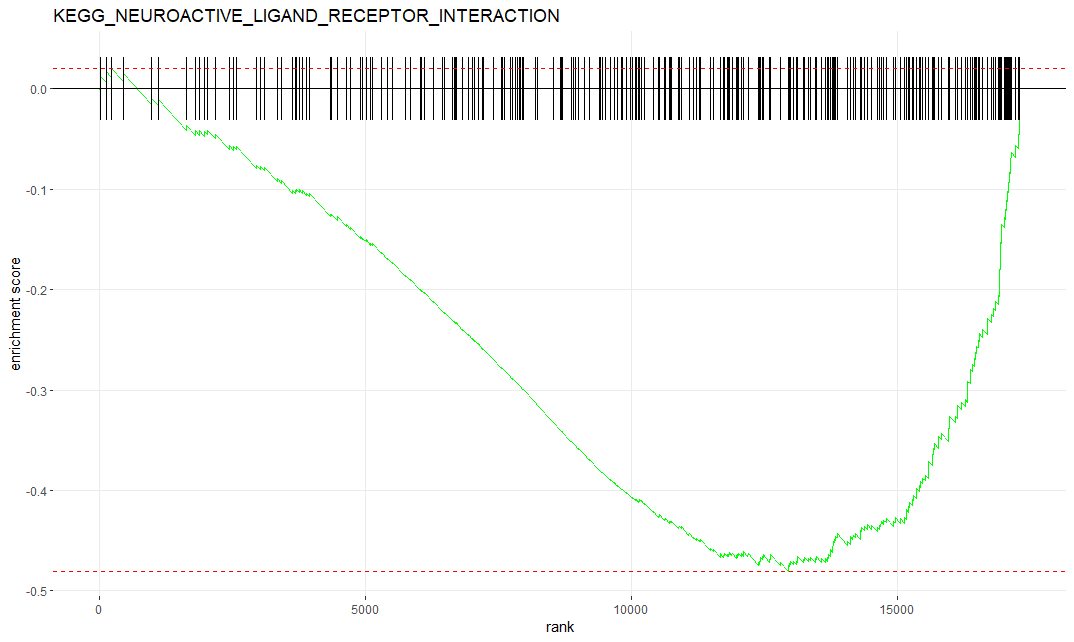
\includegraphics[width=\linewidth]{Figure/t_value.png}
		\end{figure}
	\end{frame}
	
	\subsection{Different sorting choose : T-value vs logFC}
	
	\begin{frame}{Top 10 Pathways by t-value}
		\begin{figure}[h!]
			\centering
			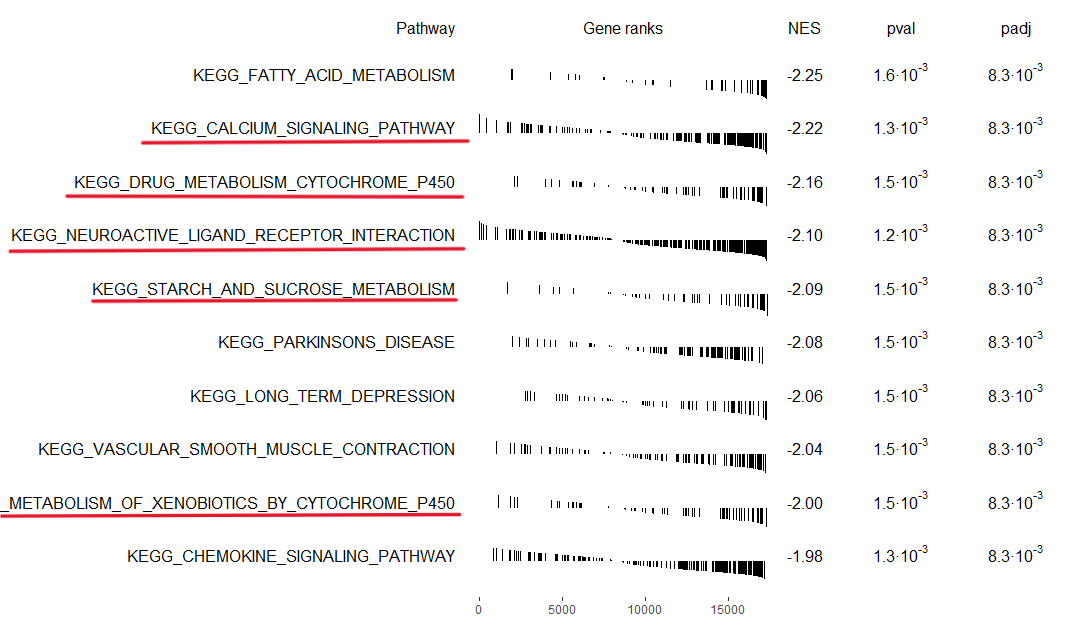
\includegraphics[width=\linewidth]{Figure/t_value_top10.png}
		\end{figure}
	\end{frame}
	
	\begin{frame}{Top 10 Pathways by logFC}
		\begin{figure}[h!]
			\centering
			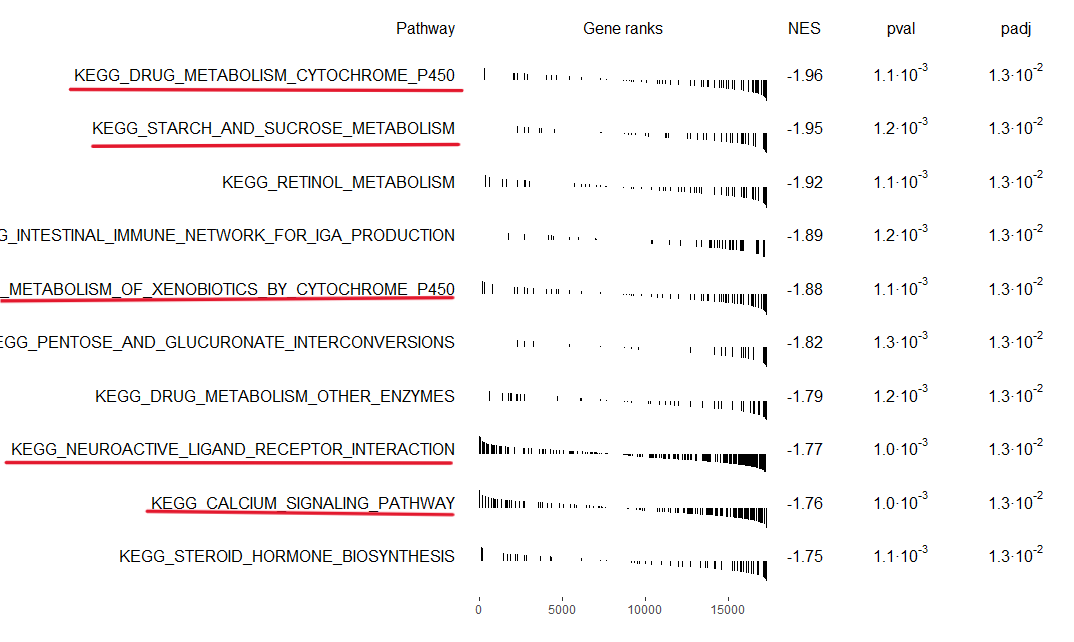
\includegraphics[width=\linewidth]{Figure/logFC_top10.png}
		\end{figure}
	\end{frame}
	

	\begin{frame}{Top Pathways}
		\scriptsize
		\begin{table}[ht]
			\centering
			\renewcommand{\arraystretch}{1.2}
			\setlength{\tabcolsep}{5pt}
			\begin{tabular}{lcccc}
				\toprule
				& \multicolumn{2}{c}{T-value} & \multicolumn{2}{c}{logFC} \\ 
				\cmidrule(lr){2-3}\cmidrule(lr){4-5}
				& padj < 0.05 & padj < 0.01 & padj < 0.05 & padj < 0.01 \\
				\midrule
				NES > 0 & 20 & 16 & 10 & 0 \\
				NES < 0 & 65 & 44 & 34 & 0 \\
				\midrule
				\textbf{Total} & \textbf{85} & \textbf{60} & \textbf{44} & \textbf{0} \\
				\bottomrule
			\end{tabular}
			\caption{Summary of enriched pathways (T-value vs logFC ranking).}
		\end{table}
		he number of pathways intersecting between T-value and logFC is $\mathbf{36}$.
	\end{frame}

	
	\begin{frame}{Top 10 Pathways by logFC}
	\scriptsize
	\begin{table}[ht]
		\centering
		\renewcommand{\arraystretch}{1.1}
		\setlength{\tabcolsep}{3pt}
		\begin{tabular}{@{}lcccc@{}}
			\toprule
			\textbf{Pathway} & \textbf{size} & \textbf{T-value leadingedge Count} & \textbf{logFC leadingedge Count} & \textbf{Common Count} \\
			\midrule
			1 & 176 & 84 & 89 & 76\\
			2 & 71 & 30 & 35 & 29\\
			3 & 270 & 116 & 98 &  95\\
			4 & 48 & 21 & 22 & 19\\
			5 & 69 & 28 & 34 & 27\\
			\bottomrule
		\end{tabular}
	\end{table}
	$\textbf{1 = KEGG\_CALCIUM\_SIGNALING\_PATHWAY}$\\
	$\textbf{2 = KEGG\_DRUG\_METABOLISM\_CYTOCHROME\_P450}$\\
	$\textbf{3 = KEGG\_NEUROACTIVE\_LIGAND\_RECEPTOR\_INTERACTION}$\\
	$\textbf{4 = KEGG\_STARCH\_AND\_SUCROSE\_METABOLISM}$\\
	$\textbf{5 = KEGG\_METABOLISM\_OF\_XENOBIOTICS\_BY\_CYTOCHROME\_P450}$\\
	\end{frame}
	
	\begin{frame}{Conclusion : logFC vs t-value}
		\begin{table}[h!]
			\centering
			\begin{tabular}{lc}
				\hline
				\textbf{Comparison Metric} & \\
				\hline
				padj & \textbf{t-value} < logFC \\
				Number of pathways (padj < 0.05) & \textbf{t-value} > logFC \\
				$|$NES$|$ &\textbf{t-value} > logFC \\
				Leading edge gene count & t-value < \textbf{logFC} \\
				\hline
			\end{tabular}
		\end{table}
		We choose t-value sorting and  
	\end{frame}
	
	
	
	\begin{frame}
		\tableofcontents[currentsection,]
	\end{frame}
	
	\subsection{Random choose and Vote}
	
	\begin{frame}{Idea}
		I have no idea how to choose the pathway.
		\vskip 0.2cm
		Initially, we consider the \textbf{K-fold} strategy. However, because pathways themselves do not serve as evaluation functions, we propose combining the results across folds using a voting mechanism, analogous to the approach employed in SVM classification.
		\vskip 0.2cm
		For each iteration, we randomly sample $r = \{0.4, 0.6, 0.8, 1\}$ of data from both Normal and Tumor groups. The \textbf{pathway with the highest adjusted p-value (padj)} is determined via a voting mechanism. This process is repeated \textbf{100 times}, and pathways appearing in more than 90 iterations are considered significant.
		
	\end{frame}
	
	
	\begin{frame}{Pathway Counts for r\_0.4}
		\scriptsize  % 或 \tiny
		\resizebox{\textwidth}{!}{
			\begin{tabular}{|c|c||c|c||c|c||c|c|}
				\hline
				Pathway & Count & Pathway & Count & Pathway & Count & Pathway & Count \\
				\hline
				1  & 3  & 2  & 2  & 3  & 1  & 4  & 4  \\
				5  & 1  & 6  & 9  & 8  & 1  & 9  & 3  \\
				15 & 1  & 18 & 1  & 21 & 1  & 30 & 1  \\
				35 & 1  & 37 & 1  & 39 & 1  & 44 & 1  \\
				45 & 1  & 50 & 1  & 51 & 1  & 62 & 1  \\
				67 & 1  & 69 & 1  & 71 & 1  & 74 & 1  \\
				77 & 1  & 81 & 1  & 82 & 1  & 90 & 1  \\
				91 & 1  & 93 & 4  & 94 & 1  & 95 & 1  \\
				96 & 1  & 97 & 1  & 98 & 1  & 99 & 1  \\
				100 & 15 & & & & & & \\
				\hline
			\end{tabular}
		}
		Number of Count > 90 is \textbf{26}
	\end{frame}
	
	\begin{frame}{Pathway Counts for r\_0.6}
		\scriptsize
		\resizebox{\textwidth}{!}{
			\begin{tabular}{|c|c||c|c||c|c||c|c|}
				\hline
				Pathway & Count & Pathway & Count & Pathway & Count & Pathway & Count \\
				\hline
				1  & 5  & 2  & 4  & 3  & 2  & 4  & 10  \\
				5  & 1  & 7  & 1  & 14 & 1  & 17 & 1   \\
				19 & 1  & 20 & 2  & 30 & 1  & 32 & 1   \\
				33 & 1  & 37 & 1  & 44 & 1  & 48 & 1   \\
				50 & 1  & 55 & 1  & 68 & 1  & 69 & 1   \\
				71 & 1  & 73 & 2  & 77 & 1  & 83 & 1   \\
				88 & 1  & 90 & 2  & 91 & 1  & 92 & 1   \\
				94 & 1  & 95 & 1  & 96 & 1  & 97 & 2   \\
				98 & 2  & 99 & 3  & 100 & 12 & & \\
				\hline
			\end{tabular}
		}
		Number of Count > 90 is \textbf{24}
	\end{frame}
	
	\begin{frame}{Pathway Counts for r\_0.8}
		\scriptsize
		\resizebox{\textwidth}{!}{
			\begin{tabular}{|c|c||c|c||c|c||c|c|}
				\hline
				Pathway & Count & Pathway & Count & Pathway & Count & Pathway & Count \\
				\hline
				1  & 2  & 2  & 3  & 4  & 5  & 5  & 2  \\
				6  & 10 & 7  & 1  & 9  & 1  & 10 & 1  \\
				13 & 1  & 15 & 1  & 17 & 1  & 23 & 1  \\
				30 & 2  & 36 & 1  & 38 & 1  & 42 & 2  \\
				43 & 1  & 53 & 1  & 61 & 1  & 62 & 1  \\
				68 & 2  & 72 & 1  & 80 & 1  & 81 & 1  \\
				82 & 1  & 86 & 1  & 89 & 1  & 90 & 1  \\
				91 & 2  & 92 & 1  & 94 & 1  & 95 & 1  \\
				96 & 1  & 97 & 4  & 98 & 1  & 100 & 13 \\
				\hline
			\end{tabular}
		}
		Number of Count > 90 is \textbf{24}
	\end{frame}
	
	\begin{frame}{Pathway Counts for r\_1}
		\scriptsize
		\resizebox{\textwidth}{!}{
			\begin{tabular}{|c|c||c|c||c|c||c|c|}
				\hline
				Pathway & Count & Pathway & Count & Pathway & Count & Pathway & Count \\
				\hline
				1  & 2  & 2  & 4  & 3  & 14 & 5  & 1  \\
				6  & 1  & 7  & 2  & 11 & 1  & 17 & 1  \\
				18 & 1  & 19 & 1  & 26 & 1  & 34 & 1  \\
				36 & 1  & 40 & 1  & 41 & 1  & 43 & 1  \\
				49 & 1  & 53 & 1  & 62 & 1  & 65 & 1  \\
				67 & 1  & 72 & 1  & 76 & 1  & 77 & 1  \\
				84 & 1  & 86 & 1  & 89 & 2  & 91 & 1  \\
				92 & 3  & 93 & 1  & 94 & 2  & 95 & 1  \\
				97 & 1  & 99 & 3  & 100 & 13 & & \\
				\hline
			\end{tabular}
		}
		Number of Count > 90 is \textbf{25}
	\end{frame}
	

	\begin{frame}{Intersection Pathways (count > 90)}
		\scriptsize
		\resizebox{\textwidth}{!}{
			\begin{tabular}{|l|}
				\hline
				KEGG\_FATTY\_ACID\_METABOLISM \\
				 KEGG\_CALCIUM\_SIGNALING\_PATHWAY \\
				KEGG\_DRUG\_METABOLISM\_CYTOCHROME\_P450 \\
				 KEGG\_PARKINSONS\_DISEASE \\
				KEGG\_STARCH\_AND\_SUCROSE\_METABOLISM \\
				\hline
				 KEGG\_NEUROACTIVE\_LIGAND\_RECEPTOR\_INTERACTION \\
				KEGG\_VASCULAR\_SMOOTH\_MUSCLE\_CONTRACTION \\
				 KEGG\_LONG\_TERM\_DEPRESSION \\
				KEGG\_METABOLISM\_OF\_XENOBIOTICS\_BY\_CYTOCHROME\_P450 \\
				 KEGG\_GNRH\_SIGNALING\_PATHWAY \\
				 \hline
				KEGG\_INTESTINAL\_IMMUNE\_NETWORK\_FOR\_IGA\_PRODUCTION \\
				 KEGG\_CHEMOKINE\_SIGNALING\_PATHWAY \\
				KEGG\_PPAR\_SIGNALING\_PATHWAY \\
				 KEGG\_VALINE\_LEUCINE\_AND\_ISOLEUCINE\_DEGRADATION \\
				KEGG\_LONG\_TERM\_POTENTIATION \\
				\hline
				 KEGG\_CARDIAC\_MUSCLE\_CONTRACTION \\
				KEGG\_PHOSPHATIDYLINOSITOL\_SIGNALING\_SYSTEM \\
				 KEGG\_ALZHEIMERS\_DISEASE \\
				KEGG\_REGULATION\_OF\_ACTIN\_CYTOSKELETON \\
				 KEGG\_ALDOSTERONE\_REGULATED\_SODIUM\_REABSORPTION \\
				\hline
			\end{tabular}
		}
	\end{frame}
	
	
		\begin{frame}{Intersection Pathways (count == 100)}
		\scriptsize
		\resizebox{\textwidth}{!}{
			\begin{tabular}{|l|}
				\hline
				KEGG\_FATTY\_ACID\_METABOLISM \\
				KEGG\_CALCIUM\_SIGNALING\_PATHWAY \\
				KEGG\_DRUG\_METABOLISM\_CYTOCHROME\_P450 \\
				KEGG\_PARKINSONS\_DISEASE \\
				KEGG\_STARCH\_AND\_SUCROSE\_METABOLISM \\
				\hline
				KEGG\_NEUROACTIVE\_LIGAND\_RECEPTOR\_INTERACTION \\
				KEGG\_VASCULAR\_SMOOTH\_MUSCLE\_CONTRACTION \\
				KEGG\_LONG\_TERM\_DEPRESSION \\
				KEGG\_METABOLISM\_OF\_XENOBIOTICS\_BY\_CYTOCHROME\_P450 \\
				KEGG\_GNRH\_SIGNALING\_PATHWAY \\
				\hline
				KEGG\_CHEMOKINE\_SIGNALING\_PATHWAY \\
				\hline
			\end{tabular}
		}
	\end{frame}
	
	
\end{document}
